% EBP course: session 4
% Thomas Klee
% 2019-02-13

% Preamble
\documentclass{beamer}
\usetheme{Singapore}
\usefonttheme[onlysmall]{structurebold}
\setbeamerfont{title}{shape=\itshape,family=\rmfamily}
\usepackage{graphicx}
\usepackage[english]{babel}
\usepackage[utf8x]{inputenc}
\usepackage{amsfonts, amsmath, amsthm, amssymb} % for math fonts, symbols and environments
\usepackage{xcolor}
\usepackage{booktabs}
\usepackage{ctable} % for command-driven tables
\usepackage{wasysym}
\usepackage[natbibapa]{apacite}
\beamertemplatenavigationsymbolsempty % uncomment to add slide navigation symbols to each slide
\setbeamertemplate{footline}[frame number]
\usepackage{appendixnumberbeamer}  % to suppress page numbers on extra slides

% activate following line for custom appearance
% \usepackage{beamerthemesplit} 

\mode<presentation>

% information for title slide
\title{Systematic Reviews \& Meta-analyses:}
\subtitle{Papers that summarize other papers}
\author{Evidence-Based Practice in Speech-Language Therapy \\ (SHSC 2033)}
\institute{Session 4}
\date{Thomas Klee \& Elizabeth Barrett}
\titlegraphic{
\includegraphics[width=6cm]{images/logo_CE_C.jpg}} % HKU logo

\begin{document}

% create title slide with information above
\begin{frame}
	\titlepage
\end{frame}

% 
\begin{frame}{Outline}
	\begin{enumerate}
	\item Systematic reviews
	\item Meta-analyses
	\item Group discussion
	\end {enumerate}
\end{frame}

% 
\begin{frame}{Clinical decision making}
	\begin{itemize}
	\item Do you really want to base a clinical decision on any one study?
	\item The more data we have on the efficacy or effectiveness of intervention, the more confidence we can have in using it with our clients.
	\end {itemize}
\end{frame}

\section*{Systematic Reviews}

%
\begin{frame}
\center{\Huge{\textcolor{darkgray}{Systematic Reviews}}}
\end{frame}

% 
\begin{frame}{Systematic reviews}
\begin{quote}
``A systematic review attempts to identify, appraise and synthesize all the empirical evidence that meets pre-specified eligibility criteria to answer a given research question. Researchers conducting systematic reviews use explicit methods aimed at minimizing bias, in order to produce more reliable findings that can be used to inform decision making." \footnote{\tiny{{\url{http://www.cochranelibrary.com/about/about-cochrane-systematic-reviews.html}}}}
\end{quote}
\end{frame}

%
\begin{frame}{Systematic reviews}
\centering

\includegraphics[width=3cm]{images/cochrane_logo_400.jpg} \\
\vspace{0.5cm}
3-minute video introduction to Cochrane reviews
\url{https://www.youtube.com/watch?v=egJlW4vkb1Y}
\end{frame}

% 
\begin{frame}{What is a systematic review?}
\begin{quote}
``\dots a form of structured literature review that addresses one or more evidence questions (or key questions) that are formulated to be answered by analysis of evidence.  Broadly, this involves:
	\begin{itemize}
	\item An objective means of searching the literature
	\item Applying predetermined inclusion and exclusion criteria to this literature
	\item Critically appraising the relevant literature
	\item Extraction and synthesis of data from evidence base to formulate answers to key questions"
	\footnote{\tiny{{\url{https://www.nlm.nih.gov/nichsr/hta101/ta10106.html}}}}
	\end{itemize}
\end{quote}
\end{frame}

% 
\begin{frame}{Simple hierarchy of intervention evidence\footnote{\tiny{\citet[p. 18]{Greenhalgh2010}}}}
	\begin{center}
	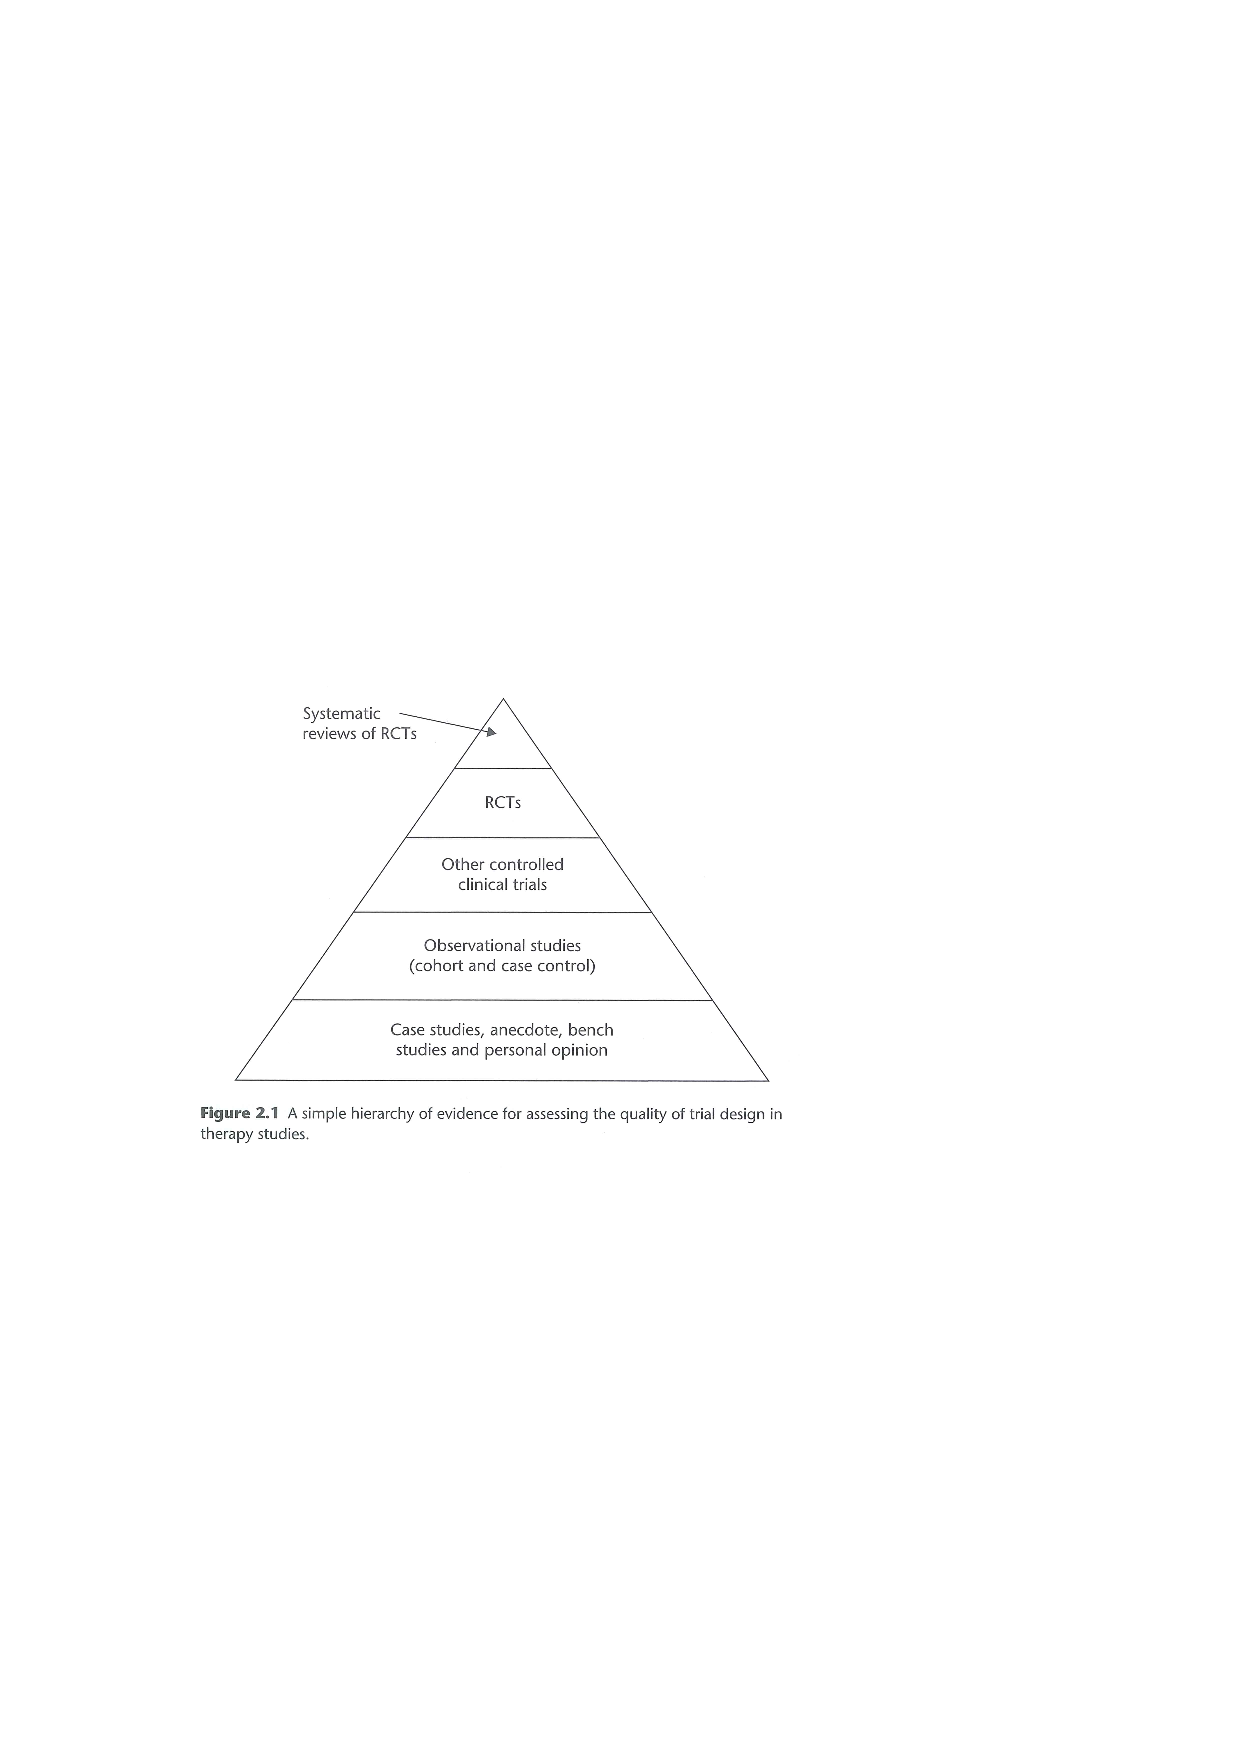
\includegraphics[width=.9\textwidth]{images/evidence_hierarchy_greenhalgh_4th.pdf}
	\end{center}
\end{frame}

% 
\begin{frame}{Levels of evidence for intervention studies\footnote{\tiny{\url{https://www.cebm.net/index.aspx?o=1025}}}}
	\begin{itemize}
	\item[1a] \alert{Systematic reviews (SR) \& meta-analyses (with homogeneity) of RCTs}
	\item[1b] Individual RCT (with narrow confidence interval)  
	\item[2a] SR (with homogeneity) of cohort studies
	\item[2b] Individual cohort study (including low quality RCT)
	\item[3a] SR (with homogeneity) of case-control studies
	\item[3b] Individual case-control studies
	\item[4] Case-series (and poor quality cohort and case-control studies)
	\item[5] Expert opinion without explicit critical appraisal; bench research
	\end{itemize}
\end{frame}

% 
\begin{frame}{Systematic reviews}
Some advantages
	\begin{itemize}
	\item You don't necessarily have to search for, read, or critically appraise (many) primary studies.
	\item SR results are based on an aggregate of primary studies (accumulated evidence).
	\item High quality SRs = highest quality evidence
	\end{itemize}
\end{frame}

% 
\begin{frame}{Systematic reviews}
Things to be aware of\ldots 
	\begin{itemize}
	\item SRs may be susceptible to \textbf{publication bias}: significant findings are more likely to be published than non-significant ones.
	\item If different kinds of interventions or outcome measures are combined, interpretation is difficult.\footnote{\tiny{For a lively discussion of this, see {\citet{Johnston2005}.}}} 
	\item SRs still need to be critically appraised, just like any other study you read.
	\item Check the publication date. If the SR is not recent, search for primary studies (e.g., RCTs) published after that to supplement the SR, so that your conclusions are up-to-date.
	\end{itemize}
\end{frame}

% 
\begin{frame}{Where to find SRs}
	\begin{itemize}
	\item \href{http://www.cochranelibrary.com/cochrane-database-of-systematic-reviews/}{Cochrane Library} (for health care research)
	\item \href{https://www.campbellcollaboration.org/}{Campbell Collaboration} (USA; for social, behavioural and educational research)
	\item \href{http://speechbite.com/}{speechBITE} (Australia; communicative disorders research; supported by SPA, ASHA, RCSLT, CASLPA CPLOL)
	\item Research journals
	\end{itemize}
\end{frame}

% 
\begin{frame}{Does Vitamin C prevent colds?}
	\begin{itemize}
	\item Controversial topic for over 70 years
	\item \href{http://onlinelibrary.wiley.com/cochranelibrary/search/}{Cochrane Library} searched using these keywords:\\``\texttt{vitamin C, colds}" 
	\item 3 SRs found; study by Hemil\"a and Chalker (2013) looks most relevant to this question.\footnote{\tiny{Searched on 2018-02-06}}
	\item Their question was: \\
	\emph{``Do oral doses of 0.2 g or more daily of vitamin C reduce the incidence, duration or severity of the common cold when used either as continuous prophylaxis or after the onset of symptoms?"}
	\end{itemize}
\end{frame}

% 
\begin{frame}{Cochrane reviews related to \\ children's speech and language disorders}
	\begin{itemize}
	\item Go to Cochrane Library website at \url{http://www.cochranelibrary.com/}
	\item Expand \texttt{Cochrane Reviews} on purple menu bar
	\item Click \texttt{Browse Reviews}
	\item Click \texttt{Developmental, psychosocial \& learning problems}
	\item Under \texttt{Filter your results}, expand \texttt{Developmental problems}
	\end{itemize}
\end{frame}

% 
\begin{frame}{Search results \footnote{\tiny{Searched on 2019-02-12}}}
Developmental, Psychosocial and Learning Problems
	\begin{itemize}
	\item Developmental problems (82)
		\begin{itemize}
		\item Autistic spectrum disorder (21)
		\item Cerebral palsy (13)
		\item Down syndrome (12)
		\item Screening for abnormalities of growth \& development (11)
		\item General neurodevelopmental problems (8)
			\begin{itemize}
			\item[-] Including SR on dysphagia in children
			\end{itemize}
		\item Speech and language disorders (7)
		\item Other (12)
		\end{itemize}
	\end{itemize}
\end{frame}

% 
\begin{frame}{Cochrane search \#2 \footnote{\tiny{Searched on 2019-02-12}}}
Keyword: ``\texttt{aphasia}"; 5 SRs found:
	\begin{itemize}
	\item 1 on speech and language therapy for aphasia (2016)
	\item 1 on transcranial stimulation for aphasia (2015)
	\item 1 on pharmacological treatment for aphasia (2001)
	\item 1 on music interventions for acquired brain injury (2017)
	\item 1 on interventions for children with primary speech and language delay or disorder (2003) \footnote{\tiny{a false positive; i.e., those with neurological damage were excluded from this review}}
	\end{itemize}
\end{frame}

% 13
\begin{frame}{Cochrane search \#3 \footnote{\tiny{Searched on 2019-02-12}}}
Record title: ``\texttt{dysphagia}"; 7 SRs found:
	\begin{itemize}
	\item 1 on patients with progressive muscle disease (2016)
	\item 1 on patients with oesophageal cancer (2014)
	\item 1 on chjildren with hereditary ataxia (2015)
	\item 1 on children with neurological impairment (2012)
	\item 1 on patients with Parkinson's disease (2001)
	\item 1 on treatment using acupuncture (2008)
	\item 1 on patients with acute and subacute stroke (2018)
	\end{itemize}
\end{frame}

% 14
\begin{frame}{Caution}
	\begin{itemize}
	\item Even though SRs of RCTs are considered to be the strongest form of intervention evidence, \alert{they still need to be critically appraised}.
	\item Use CASM rather than CATE \citep{Dollaghan2007}.
	\item Look at the publication date of the SR. You may need to also search for newer primary studies to make sure your conclusion is up-to-date.	
	\end{itemize}
\end{frame}

\section*{Meta-Analyses}

%
\begin{frame}
\center{\Huge{\textcolor{darkgray}{Meta-Analyses}}}
\end{frame}

% 
\begin{frame}{Meta-analyses}
	\begin{itemize}
	\item Many SRs contain meta-analyses—a statistical method that summarizes the findings of two or more primary studies.
	\item \emph{``\ldots a statistical synthesis of the numerical results of several trials which all addressed the same question"} \footnote{\tiny{\citet[p. 121]{Greenhalgh2010}}}
	\item \emph{``Systematic methods that use statistical techniques for combining results from different studies to obtain a quantitative estimate of the overall effect of a particular intervention or variable on a defined outcome. This combination may produce a stronger conclusion than can be provided by any individual study.''} \footnote{\tiny{https://www.nlm.nih.gov/nichsr/hta101/ta101014.html}}
	\item Think of MAs as quantitative SRs.
	\end{itemize}
\end{frame}

% 
\begin{frame}{Meta-analyses are cool \smiley}
\emph{``A good meta-analysis is often easier for the non-statistician to understand than the stack of primary research papers from which it was derived.
\\
\ldots the underlying statistical techniques used for meta-analysis are exactly the same as the ones for any other data analysis--it's just that the numbers are bigger."} \footnote{\tiny Greenhalgh (2010, p. 121)}
\end{frame}

% 
\begin{frame}{Statistical analyses in MAs}
	\begin{itemize}
	\item Most MA results are presented in a standard way.
	\item Results of \alert{included studies} are graphed using a \textbf{forest plot}. 
		\begin{itemize}
		\item Effect size (ES) and 95\% CI are plotted for each study.
		\item Vertical line represents \alert{no treatment effect}. ES with CI that crosses this is regarded as non-significant.
		\item Results are then combined to produce an \alert{overall estimate of effect size} and depicted as a $\Diamond$ diamond in the graph.
		\end{itemize}
	\end{itemize}
\end{frame}

% 
\begin{frame}{Forest plot  \\ \scriptsize{From \citet[p. 3]{Law2004a}}}
\begin{center}
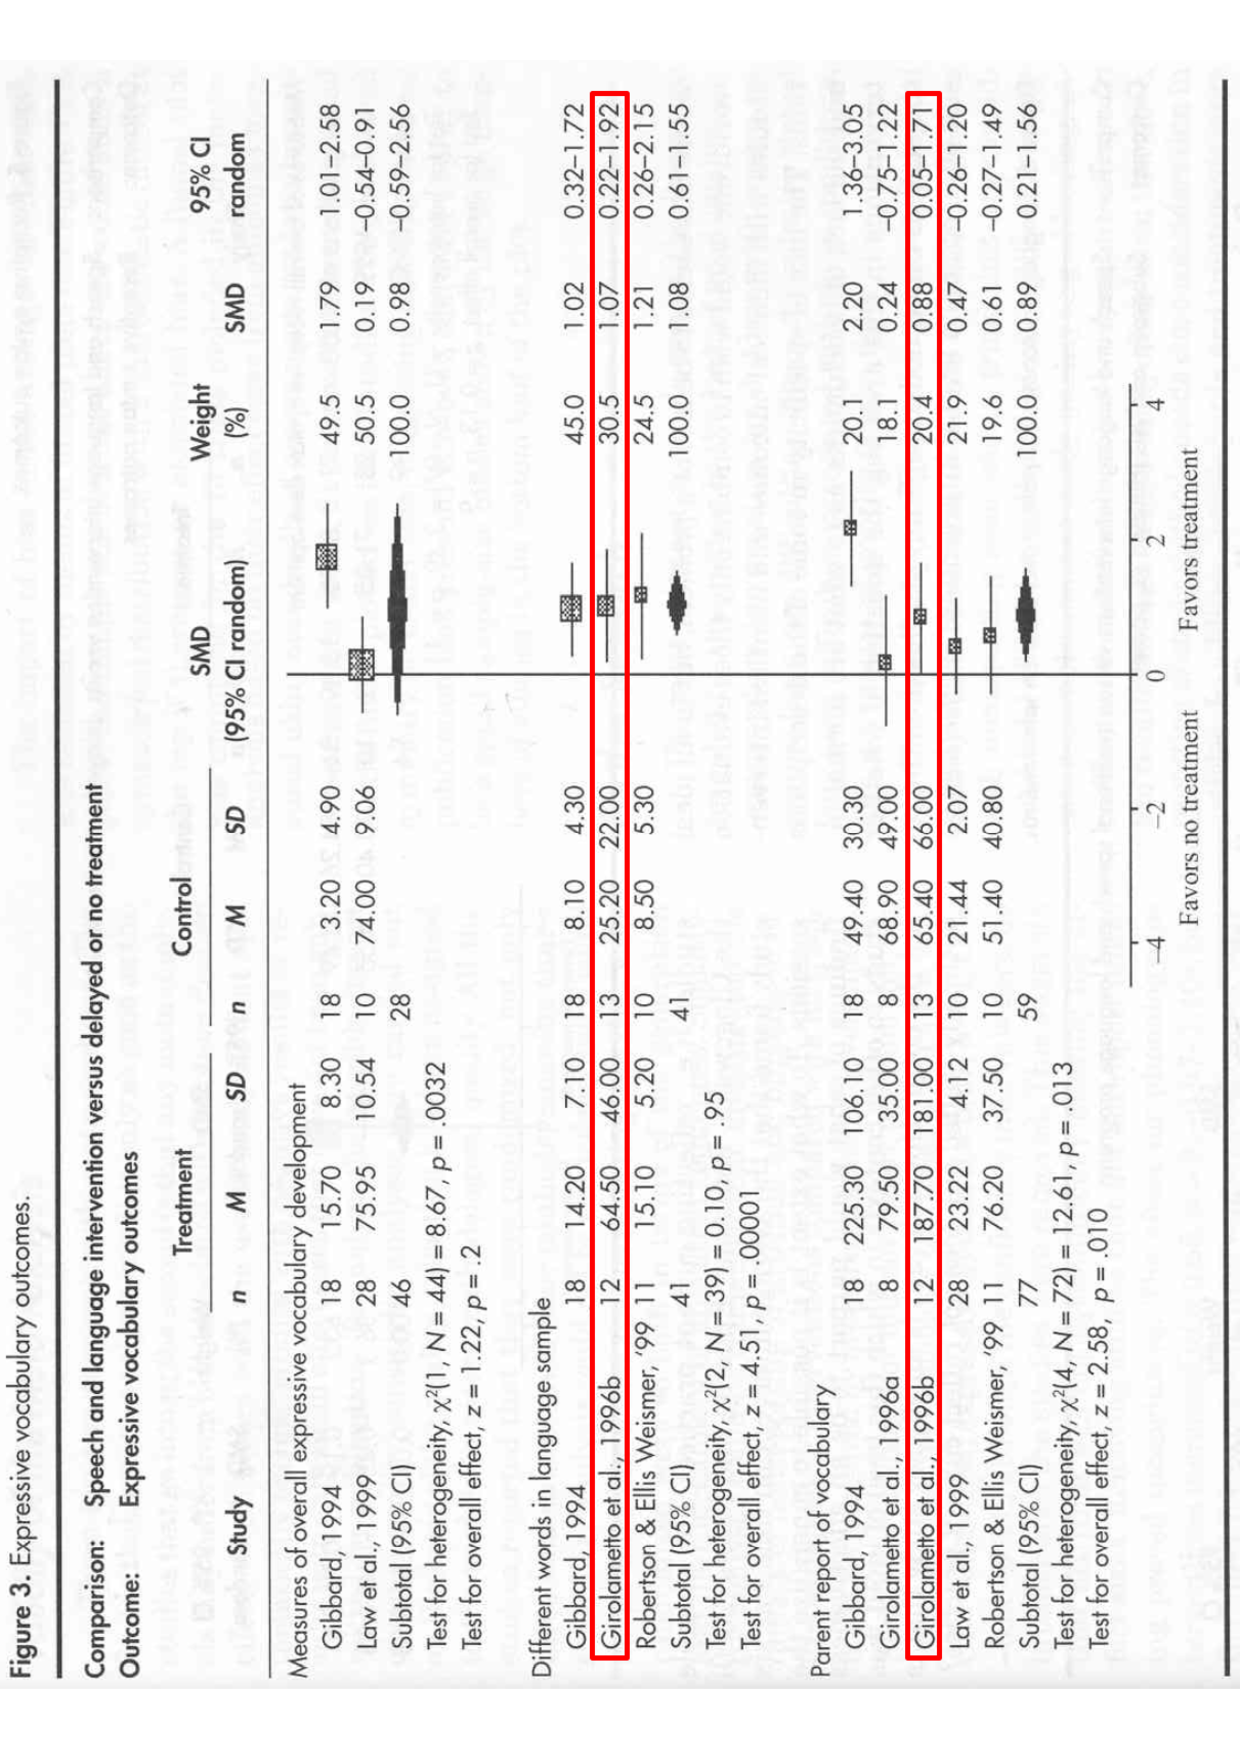
\includegraphics[angle=270, origin=c, width=10cm]{images/law_fig3a.pdf}
\end{center}
\end{frame}

% 
\begin{frame}{Forest plot  \\ \scriptsize{From \citet[p. 3]{Law2004a}}}
\begin{center}
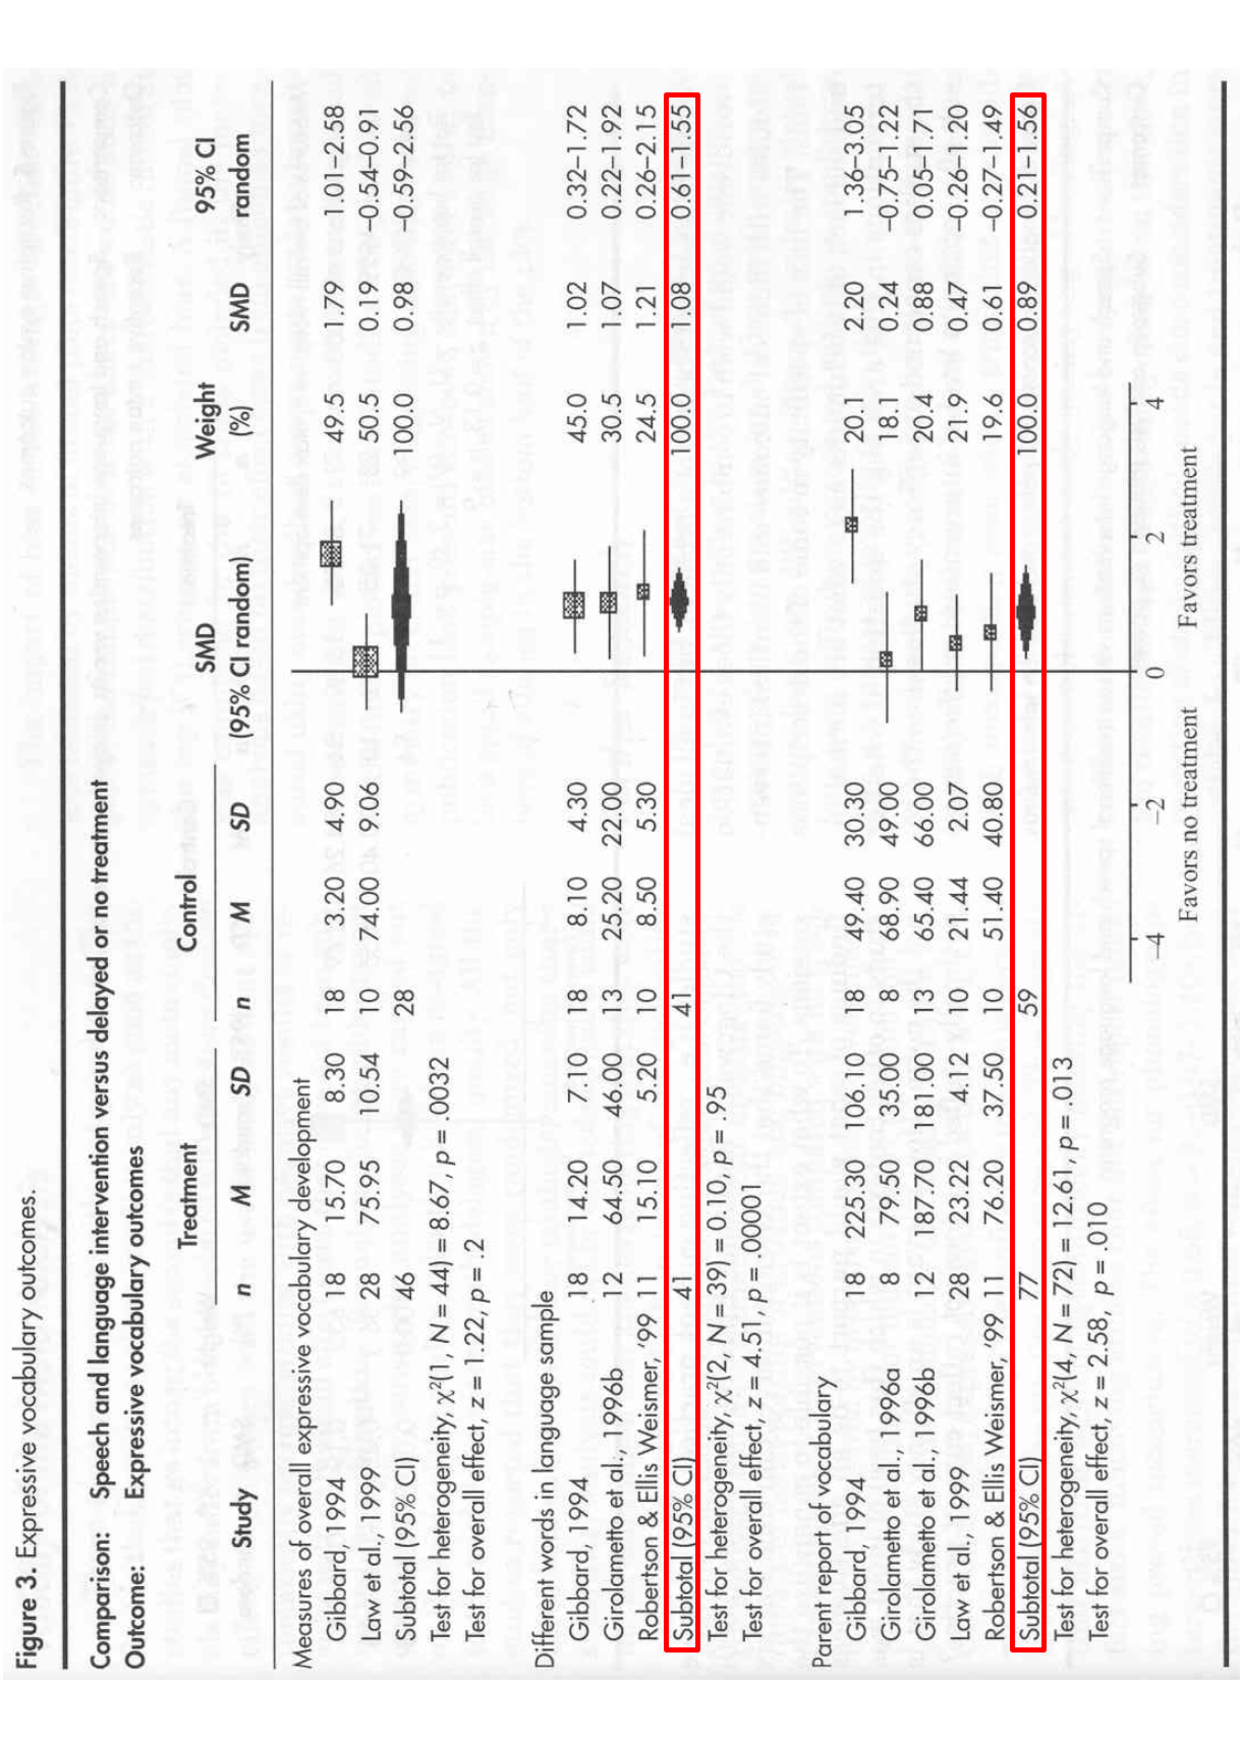
\includegraphics[angle=270, origin=c, width=10cm]{images/law_fig3b.pdf}
\end{center}
\end{frame}

% 
\begin{frame}{Conclusions based on a meta-analysis \footnote{\tiny{Law et al. (2004)}}}
	\begin{itemize}
	\item Intervention is effective in certain areas.
	\item Across studies, treated groups had significantly better expressive vocabulary outcomes than control groups.
		\begin{itemize}
		\item NDW in language sample: \emph{d} = 1.08, 95\% CI [.61, 1.55]
		\item Parent-reported vocabulary: \emph{d} = .89, 95\% CI [.21, 1.56]
		\item Notice that \alert{standardized ESs} are reported above.
		\end{itemize}
	\end{itemize}
\end{frame}

% 
\begin{frame}{Useful tools}
	\begin{enumerate}
	\item Prospective study registration for authors of SRs and MAs: \\ \alert{PROSPERO} (\url{https://www.crd.york.ac.uk/prospero/})
	\item Reporting standards for authors of SRs and MAs: \\ \alert{PRISMA} (\url{www.prisma-statement.org})
	\item Critical appraisal checklist for readers of SRs and MAs: \\ \alert{CASM} (Dollaghan, 2007, p. 157)
	\end{enumerate}
\end{frame}

% 
\begin{frame}{ASHA's evidence maps}
	\begin{itemize}
	\item Summaries of clinical research related to assessment and intervention in communication disorders
	\item Contain published SRs that are not in the Cochrane Library. 
	\item See \url{http://on.asha.org/evidence-maps}
	\item Also, see \url{http://www.asha.org/Research/EBP/EBSRs}
	\end{itemize}
\end{frame}

% 
\begin{frame}{\alert{Cherry picking}}
	\begin{itemize}
	\item Choosing what you want to believe by ignoring some studies or not critically appraising them.
	\item This can result from believing what you read in the popular press or relaying on information from web sites with an axe to grind.
	\item Example: Not having your child vaccinated because \emph{``MMR vaccine causes autism."} 
	\item Searching for, and critically appraising the evidence, should help you avoid this cognitive error. 
	\end{itemize}
\end{frame}

\section*{Group Discussion}

% 
\begin{frame}{Group discussion}
	\begin{itemize}
	\item Break up into your assigned groups.
	\item Use CASM (Dollaghan, 2007, p. 157) to critically appraise the research article.
	\item Document \alert{where} you found information addressing each point.
	\end{itemize}
\end{frame}

%
\begin{frame}%[allowframebreaks] %[shrink=15] % to reduce font size of references
	\frametitle{References}
	\bibliographystyle{apacite}
	\small\bibliography{/Users/thomasklee/Documents/Bibtex/library}
\end{frame}

\end{document}
